F\"ur   die  Regler-Dimensionierung   sowie  das   grafische  Darstellen   der
Schrittantwort  muss   die  Software  einige  Berechnungen   ausf\"uhren.   Im
folgenden  Kapitel werden  die wichtigsten  Schritte dieser  Berechnungen kurz
zusammengefasst und erkl\"art.

\begin{itemize}
    \item
    Bestimmung  des  Frequenzgangs  der  Regelstrecke  aus  Verz\"ogerungszeit
    $T_u$, Anstiegszeit $T_g$ und Verst\"arkung $K_s$.
    \item
    Dimensionierung des Reglers mittels Faustformeln.
    \item
    Dimensionierung des Reglers durch Phasengangmethode.
    \item
    Umrechung der Regler-Darstellung zwischen bodekonformer und reglerkonformer
    Darstlelung. \todo{Erkl\"arung}
    \item
    Berechnung der Schrittantwort des geschlossenen Regelkreises.
\end{itemize}

\subsection{Frequenzgang der Regelstrecke}
Im   Praxiseinsatz  stehen   f\"ur   die  Dimensieung   der  Regler   einfache
Berechnungsformeln f\"ur die Einstellwerte der  Regler anhand von $T_u$, $T_g$
und $K_s$ zur Verf\"ugung.

Einige   dieser  Faustformeln   werden  in   der  Applikation   zum  Vergleich
mitberechnet. Die    dazugeh\"origen    Berechnungen    sind    der    Tabelle
\ref{tab:faustformeln} zu entnehmen.

\begin{longtable}{p{50mm}rrrrr}
    \toprule

    %\multicolumn{3}{l}{\large{\textsc{Auftragsanalyse und Hintergrundinformationen}}} \\

    Faustformel
    &
    \multicolumn{2}{l}{PI-Regler}
    &
    \multicolumn{2}{l}{PID-T1-Regler}
    \\

    &
    $T_n$
    &
    $K_p$
    &
    $T_n$
    &
    $T_v$
    &
    $K_p$
    \\

    \midrule

    \endhead
    \endfoot
    \endlastfoot

    % CONTENT HERE ---------------------------------------------------------- %

    \pbox{45mm}{Chiens, Hrones, Reswick \\ \small{\textbf{(0\% \"Uberschwingen)}} \\ \cite{ref:chiens_tsn}, \cite{ref:chiens_wiki}}
    &
    $1.2\cdot T_g$
    &
    $\frac{0.35}{K_s} \cdot \frac{T_g}{T_u}$
    &
    $T_g$
    &
    $0.5\cdot T_u$
    &
    $ \frac{0.6}{K_s} \cdot \frac{T_g}{T_u} $
    \\

    \addlinespace[1em]

    \pbox{45mm}{Chiens, Hrones, Reswick \small{\textbf{(20\% \"Uberschwingen)}} \\ \cite{ref:chiens_tsn}, \cite{ref:chiens_wiki}}
    &
    $T_g$
    &
    $\frac{0.6}{K_s} \cdot \frac{T_g}{T_u}$
    &
    $1.35\cdot T_g$
    &
    $0.47 \cdot T_u$
    &
    $ \frac{0.95}{K_s} \cdot \frac{T_g}{T_u} $
    \\

    \addlinespace[1em]

    Oppelt \cite{ref:op_ros_zieg}
    &
    $3 \cdot T_u$
    &
    $\frac{0.8}{K_s} \cdot \frac{T_g}{T_u}$
    &
    $2 \cdot T_u$
    &
    $ 0.42 \cdot T_u $
    &
    $ \frac{1.2}{K_s} \cdot \frac{T_g}{T_u} $
    \\

    \addlinespace[1em]

    Rosenberg \cite{ref:op_ros_zieg}
    &
    $3.3 \cdot T_u $
    &
    $ \frac{0.91}{K_s} \cdot \frac{T_g}{T_u} $
    &
    $ 2 \cdot T_u $
    &
    $ 0.45 \cdot T_u $
    &
    $ \frac{1.2}{T_s} \cdot \frac{T_g}{T_u}$
    \\

    \addlinespace[1em]

    Ziegler/Nichols \cite{ref:op_ros_zieg}
    &
    $ 3.33 \cdot T_u $
    &
    $ \frac{0.9}{K_s} \cdot \frac{T_g}{T_u} $
    &
    $ 2 \cdot T_u $
    &
    $ 0.5 \cdot T_u $
    &
    $ \frac{1.2}{K_s} \cdot \frac{T_g}{t_u} $
    \\

    \bottomrule
\caption{Faustformeln zur Reglerdimensionierung}
\label{tab:faustformeln}
\end{longtable}
\todo{Quellen hinzuf\"ugen}


\subsection{Regler-Dimensionierung mittels Faustformeln}
\todo{N\"ahere Erl\"auterungen?}
\todo{Bildliche  Illustration   einer  Schrittantwort  der  Strecke   und  des
zugeh\"origen Frequenzgangs?}

F\"ur  die   Identifikation  des   Freqeunzgangs  steht   die  Matlab-Funktion
\code{p2\_sani.m} zur  Verf\"ugung, welche in  der Lage ist, PTn  Strecken mit
einem Grad zwischen 1 und 8 zu identifizieren. Deshalb wird hier nicht n\"aher
auf  die  Berechnung  eingegangen,  da die  Funktion  lediglich  in  Java-Code
``\"ubersetzt'' werden muss.


\subsection{Regler-Dimensionierung durch Phasengangmethode}
Die    Aufgabe   eines    geschlossenen    Regelkreises (Abbildung \ref{fig:geschlossenerRegelkreis}) ist  es, einen  vorgegeben Sollwert  zu erreichen  und diesen
auch bei  St\"orungen aufrecht zu  erhalten. Dabei sollen die  unten genannten
dynamischen  Anforderungen  eingehalten  werden, damit  die  Stabilit\"at  des
Regelsystems garaniert ist. Die wichtigste  Bedingung f\"ur die Schrittantwort
ein  geschlossenen  Regelkreis heisst,  dass  der  Regelfehler, die  Differenz
zwischen Ist-und Sollwert, gleich Null oder m\"oglichst klein ist.\\


\begin{figure}[!h!, width=\pagewidth]
\begin{center}
    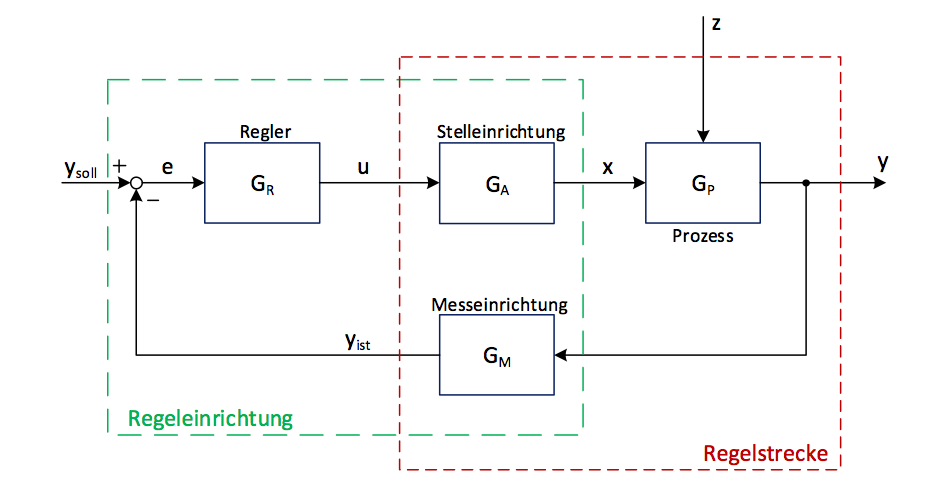
\includegraphics[width=0.5\textwidth]{images/geschlRegelkreis}
    \caption{Geschlossener Regelkreis}
    \label{fig:geschlossenerRegelkreis}
\end{center}
\end{figure}

%Name Bild Struktur eines allgemeinen Regelkreises
\begin{itemize}
    \item
        $y_soll$ bezeichnet den Sollwert der Regelgr\"osse.
    \item
        $e$ Regelabweichung (Regelfehler)
    \item
        $u$ Steuergr\"osse
    \item
        $x$ Stellgr\"osse
    \item
        $y$ Regelgr\"osse
    \item
        $z$ St\"orgr\"osse
    \item
        $y_ist$  ist der  Ist-Wert der  Regelgr\"osse  und wird  auch als  die
        Schrittantwort des Regelkreis bezeichnet.
\end{itemize}

\todo{Bild Schrittantworten passend zu Aufzählung unten}

Grunds\"atzlich  k\"onnen  f\"unf   Anforderungen  f\"ur  einen  geschlossenen
Regelkreis und deren Schrittantworten zusammengefasst werden:\\
\begin{enumerate}
    \item Der Regelkreis muss stabil sein:
        \begin{itemize}
            \item
                Das heisst  f\"ur die Schrittantwort, dass  nach dem Erreichen
                des  eingeschwungenen  Zustand kein  erneutes  \"Uberschwingen
                stattfinden darf.
            \item
                F\"ur  das  Regelsystem  heisst  stabil,  dass  es  in  seinen
                Gleichgewichtszustand zur\"uckgef\"uhrt werden kann.
        \end{itemize}
    \item
        Der Regelkreis  muss gen\"ugend ged\"ampft sein: \\Die  D\"ampfung der
        Schrittantwort soll  so stark  sein, dass der  eingeschwungene Zustand
        m\"oglichst  rasch erreicht  wird  ohne dass  das \"Uberschwingen  des
        Systems zu stark wird.
    \item
        Der   Regelkreis   muss   eine  bestimmte   station\"are   Genauigkeit
        aufweisen: Das  bedeutet,  der  Regelfehler  e(t) soll  f\"ur  t->  oo
        gegen  Null  gehen. F\"ur  die  Schrittantwort heisst  das,  dass  die
        Schrittantwort gleich $y_soll$ sein muss.
    \item
        Der Regelkreis  muss hinreichend  schnell sein: Die  Schnelligkeit des
        Einschwingvorganges der  Schrittantwort ist  stark von  der D\"ampfung
        abh\"angig. Ist die D\"ampfung  zu stark oder zu  schwach, braucht der
        Einschwingvorgang mehr Zeit. Hierbei muss darauf geachtet werden, dass
        die spezifischen Anforderungen an das Regelsystem eingehalten werden.
    \item
        Der  Regelkreis muss  robust  sein: Der Regelkreis  muss so  ausgelegt
        werden,  dass  das  Regelsystem  auch im  schlimmsten  Fall  (je  nach
        Regelsystem situationsabh\"angig) in der Lage ist, das System zur\"uck
        in den stabilen Zustand (vgl. 1.) zu regeln.
\end{enumerate}


\subsection{Umrechnung zwischen bodekonformer und reglerkonformer Darstellung}
Als     Hauptberechnung    wird     die    sogenannte     ``Phasengang-Methode
zur      Reglerdimensionierung''      von     Jakob      Zellweger      (FHNW)
\cite{regelungstechnik:zellweger_short}   zu   Hilfe   genommen. Diese   wurde
urspr\"unglich  als  vereinfachte  grafische  Methode  zur  Approximation  der
-20dB/Dek Methode erarbeitet und soll im Rahmen dieses Projektes automatisiert
werden. Schlussendlich   soll   sie   zur   numerischen   Berechnung   mittels
N\"aherungen in das Tool implementiert sein.

Um die  Berechnung mit  der Phasengang-Methode  zu erm\"oglichen,  muss zuerst
die  vermessene  Regelstrecke  in   eine  Funktion  im  Bildbereich  gewandelt
werden. Dazu  wird die  bereits  erw\"ahnte Matlab-Funktion  \code{p2\_sani.m}
verwendet  \todo{Ist  dies  bezogen  auf  das  schlussendliche  Programm  noch
korrekt? Falls nein,  anpassen}. Die Berechnung anhand  der Phasengang-Methode
wird  nachfolgend  als  Rezept aufgef\"uhrt. Genauere  Informationen  sind
dem   Skript   \cite{regelungstechnik:zellweger_short}  zu   entnehmen.    Das
\"Uberschwingverhalten  des Regelkreises  soll  f\"ur dieses  Projekt in  drei
Stufen berechnet werden. Verwendet wird dazu folgende Abstufung:
\todo{Ist diese Einteilung des \"Uberschwingens noch aktuell oder wurde das
in der Auftragserweiterung angepasst?}


\begin{itemize}
    \item
        wenig \"Uberschwingen (ca. 0\%)
    \item
        mittleres \"Uberschwingen (ca. 16\%)
    \item
        starkes \"Uberschwingen (ca. 23\%)
\end{itemize}

\subsubsection{Rezept}
Als Erstes sollten folgende Begriffe definiert werden:
\begin{longtable}{lp{60mm}}
    \toprule
    \endhead
    \endfoot
    \endlastfoot

    % CONTENT HERE ---------------------------------------------------------- %

    $H_s(j\omega)                                                                   $ &  \"Ubertragungsfunktion der Regelstrecke \\
    $A_s(j\omega)=|H_s(j\omega)|                                                    $ &  Amplitudengang der Regelstrecke \\
    $\varphi_s(j\omega)=arg(H_s(j\omega))                                           $ &  Phasengang der Regelstrecke \\
    $H_r(j\omega)                                                                   $ &  \"Ubertragungsfunktion des Reglers \\
    $A_r(j\omega)=|H_r(j\omega)|                                                    $ &  Amplitudengang des Reglers \\
    $\varphi_r(j\omega)=arg(H_r(j\omega))                                           $ &  Phasengang des Reglers \\
    $H_o(j\omega)=H_s \cdot H_r(j\omega)                                            $ &  \"Ubertragungsfunktion des nicht geschlossenen Regelkreises \\
    $A_o(j\omega)=|H_o(j\omega)|                                                    $ &  Amplitudengang des nicht geschlossenen Regelkreises \\
    $\varphi_o(j\omega)=arg(H_o(j\omega))=\varphi_s(j\omega)+\varphi_r(j\omega)     $ &  Phasengang des nicht geschlossenen Regelkreises \\
    $H_{rpid}= K_{rk}\Big[ \frac{(1+sT_{nk})(1+sT_{vk})}{sT_{nk}}\Big]              $ & \"Ubertragungsfunktion des PID-Reglers \\
    $H_{rpi} = K_{rk}\Big[ 1 + \frac{1}{sT_{nk}} \Big] $ & \"Ubertragungsfunktion des PI-Reglers \\


    \bottomrule
    %\caption{Caption here}
\end{longtable}

\clearpage
\subsubsection{Rezept PID-Regler}
\todo{Grafische Illustration der Rezepte? W\"urde es der Leserin erleichtern,
sich ein Bild des Prozesses zu machen, speziell da die Phasengangmethode
ja im Kern eine grafische Methode ist.}


\begin{enumerate}
    \item
        Im  Phasengang muss  die  Frequenz  $\omega_{pid}$ gem\"ass  Gleichung
        \ref{eq:phi_s} bestimmt werden \footnotemark[1].
        \begin{equation} \label{eq:phi_s}
            \varphi_s(\omega_{pid}) = -135 \degree.
        \end{equation}
    \item
        Mittels  Ableitung  wird  die  Steigung des  Phasengangs  im  Punkt  $
        \omega_{pid} $ bestimmt.
    \item
        $\beta$ ist so w\"ahlen, dass Gleichung \ref{eq:dphi_o} erf\"ullt ist

        \begin{equation} \label{eq:dphi_o}
            \frac{d\varphi_o}{d\omega_{pid}}= -\frac{1}{2}.
        \end{equation}

        wobei:
        \vspace*{1em}

        \begin{center}
            $\frac{\omega_{pid}}{\beta}=\frac{1}{T_{vk}}$,
            $\omega_{pid} \cdot \beta=\frac{1}{T_{nk}}$,
            $T_p = 0$,
            $K_{rk} = 1$
        \end{center}

        \vspace*{1em}
        {\em{Man Beachte: Falls $\beta$ komplex werden sollte, muss $\beta=1$ gesetzt werden.}}
        \vspace*{1em}
    \item
        Nun   werden    $T_{vk}$,   $T_{nk}$   sowie   $K_{rk}=1$    in   die
        \"Ubertragungsfunktion  $H_r$  eingesetzt. Daraus folgen  $\varphi_o$
        sowie $A_o$.   Je nach  gew\"unschtem \"Uberschwingverhalten  wird der
        entsprechende Wert  f\"ur $\varphi_s$ aus der  Tabelle \ref{tab:phi_s}
        herausgelesen.

        Durch Suchen des Punktes  $\omega_d$ gem\"ass Gleichung \ref{eq:phi_o}
        wird berechnet, an welchem Punkt  f\"ur $A_o$ eine Verst\"arkung von 1
        herrschen muss.

        \begin{equation} \label{eq:phi_o}
            \varphi_o(\omega_d)=\varphi_s.
        \end{equation}

        \begin{longtable}{llll}
            \toprule
            \endhead
            \endfoot
            \endlastfoot

            % CONTENT HERE ---------------------------------------------------------- %

            \"Uberschwingen & 0\%              & 16.3\%           & 23.3\% \\
            $\varphi_s$        & $-103.7 \degree$ & $-128.5 \degree$ & $-135 \degree$ \\

            \bottomrule
            \caption{Werte f\"ur $\varphi_s$}
            \label{tab:phi_s}
        \end{longtable}

    \item
        Durch geeignete Wahl von  $K_{rk}$ mithilfe von Gleichung \ref{eq:A_o}
        eine Verst\"arkung von 1 erzwingen:

        \begin{equation} \label{eq:A_o}
            A_o(\omega_d) \cdot K_{rk} = 1
        \end{equation}

    \item
        Alle  Freiheitsgrade des  PID-Reglers  sind hiermit  bestimmt und  der
        Regler nach der Phasengang-Methode vollst\"andig dimensioniert.
\end{enumerate}

\footnotetext[1]{Der Winkel stellt keinen endg\"ultigen Wert dar. Dieser wurde von Jakob Zellweger fixiert, um eine grafische Evaluation \"uberhaupt zu erm\"oglichen. Durch \"andern dieses Wertes kann je nach Regelstrecke das
Regelverhalten weiter optimiert werden.}


\subsubsection{Rezept PI-Regler}

\begin{enumerate}
    \item
        Im  Phasengang  muss  die Frequenz  $\omega_{pi}$  gem\"ass  Gleichung
        \ref{eq:phi_s_pi} bestimmt werden \footnotemark[1].

        \begin{equation} \label{eq:phi_s_pi}
            \varphi_s(\omega_{pi})=-90 \degree.
        \end{equation}

    \item
        $T_{nk}$ kann dadurch direkt bestimmt werden.
        \begin{equation} \label{eq:Tnk_pi}
            T_{nk}=\frac{1}{\omega_{pi}}.
        \end{equation}

    \item
        Anschliessend    werden    $T_{nk}$     und    $K_{rk}=1$    in    die
        \"Ubertragungsfunktion $H_r$  eingesetzt, was $\varphi_o$  sowie $A_o$
        liefert. Jetzt  muss  je  nach gew\"ahltem  \"Uberschwingverhalten  der
        entsprechende Wert  f\"ur $\varphi_s$ aus der  Tabelle \ref{tab:phi_s}
        herausgelesen werden.

        Durch Suchen des Punktes  $\omega_d$ gem\"ass Gleichung \ref{eq:phi_o}
        wird festgelegt an  welchem Punkt f\"ur $A_o$ eine  Verst\"arkung von 1
        definiert werden muss.

    \item
        $K_{rk}$ wird  so gew\"ahlt, dass mithilfe  von Gleichung \ref{eq:A_o}
        eine Verst\"arkung von 1 erzwungen wird.

    \item
        Somit sind alle Freiheitsgrade des  PI-Reglers bestimmt und der Regler
        nach der Phasengang-Methode komplett dimensioniert.
\end{enumerate}


\subsection{Schrittantwort des geschlossenen Regelkreises}
Die    Formeln   in    Tabelle   \ref{tab:bode_regler_konform}    dienen   zur
Umrechnung  zwischen der  bodekonformen  Darstellung  und der  reglerkonformen
Darstellung. N\"ahere  Informationen  zu den  verschiedenen  Darstellungsarten
k\"onnen der Quelle \cite{regelungstechnik:zellweger} entnommen werden.
\todo{Allenfalls noch  ein paar kurze  S\"atze zum Sinn  dieser \"Ubung? Sonst
wird nirgends  darauf wirklich  Bezug genommen, Abschnitt  ist ein  wenig ohne
Kontext in der Landschaft.}

\begin{longtable}{l|ll}
    \toprule

    %\multicolumn{3}{l}{\large{\textsc{auftragsanalyse und hintergrundinformationen}}} \\
    %\multicolumn{2}{l}{pi}

    &
    bodekonform $\rightarrow$ reglerkonform
    &
    reglerkonform $\rightarrow$ bodekonform
    \\

    \midrule

    \endhead
    \endfoot
    \endlastfoot

    % content here ---------------------------------------------------------- %

    PI
    &
    $T_n = T_{nk} $ %reglerkonform
    &
    $K_{rk} = K_r $ %bodekonform
    \\

    \midrule

    PID
    &
    $T_n = T_{nk}+T_{vk}-T_p$
    &
    $T_{nk}=0.5 \cdot (T_n+T_p) \cdot (1+\epsilon)$
    \\

    &
    $T_v=\frac{T_{nk} \cdot T_{vk}}{T_{nk}+T_{vk}-T_p}-T_p$
    &
    $T_{vk}=0.5 \cdot (T_n+t_p) \cdot (1-\epsilon)$
    \\

    &
    %$k_r=k_{rk} \cdot \frac{1+t_{vk}}{t_{nk}}$
    $K_r=K_{rk} \cdot (1 + \frac{T_{vk}-T_p}{T_{nk}})$
    &
    $K_{rk} = 0.5 \cdot K_r \cdot (1 + \frac{T_p}{T_{nk}}) \cdot (1+\epsilon )$
    \\
    \\

    &
    \multicolumn{2}{l}{wobei $\epsilon^2 = 1-(4 \cdot T_n \cdot \frac{T_v-T_p}{(T_n+T_p)^2})$}
    \\
    \bottomrule
    \caption{Formeln zur Umrechung zwischen bode- zu reglerkonformer Darstellung \cite{regelungstechnik:zellweger}, \cite{regelungstechnik:schumleon}}
    \label{tab:bode_regler_konform}
\end{longtable}


F\"ur die Berechnungen in diesem Projekt wird, wenn nicht anders angegeben, mit $T_p=\frac{1}{10} \cdot T_v$ gerechnet.

